\documentclass[12pt,openright]{report}
\pagestyle{headings}
\usepackage{layout} 
\usepackage[left=1.4in, right=1.0in, top=1.2in, bottom=1.2in]{geometry} %page margin


\usepackage[utf8]{inputenc}
%\usepackage[brazil]{babel}
%\usepackage{biblatex} %Bibliografia. Cita sites
\usepackage{url}
%%%%%%%%%%%%%%%%%%%%%%%%
%\usepackage[latin1]{inputenc} -> separação de silabas


%\usepackage{pslatex} %Times New Roman Font 
\usepackage{fontenc}
\usepackage{verbatim} %inclui comentários em blocos
\usepackage{indentfirst} %primeiro paragrado identado

%%%%%%%%%%%%%%%%%%%% simbolos matematicos
\usepackage[intlimits]{amsmath} %limites do lim ficam embaixo!
\usepackage{amsthm, amssymb} 
%%%%%%%%%%%%%%%%%%%

%%%%%%%%%%%%%%%%%%%% fontes matematicas
\usepackage{amsfonts, mathrsfs} 
%\usepackage{bbold} % modifica o \mathbb para fazer matriz identidade
%%%%%%%%%%%%%%%%%%%


\usepackage{graphicx,color,array}
\usepackage{float} %para usar comando [H] na fig e posicionar figuras onde quero
%\usepackage{mathtools} %inclui automaticamente o 'amsmath'
\usepackage{multicol}

%\usepackage{mathtools} %inclui automaticamente o 'amsmath'

\usepackage{ctable}

%\usepackage{natbib} % bibliography style file

%%%%%%%%%%%%%%%%%%%% esteticos
\setlength{\belowcaptionskip}{10pt} %espaço abaixo do caption
%%%%%%%%%%%%%%%%%%%


\usepackage[portuguese,ruled,vlined,linesnumbered,boxed]{algorithm2e} % Pacote para escrever algoritmos em Portugol
\renewcommand{\algorithmautorefname}{Algoritmo}% para utilizar \autoref

% Adicione o trecho a seguir somente se desejar incluir uma Lista de algoritmos (opcional)
%\renewcommand{\listalgorithmcfname}{Lista de algoritmos}%
%\renewcommand{\listasdousuario}{
%  \pdfbookmark[0]{\listalgorithmcfname}{loa}
%  \listofalgorithms
%  \cleardoublepage
%}




%%%%%%%%%%%%%%%%%%% não estão sendo usados!
%\usepackage{tikz}      %gera fluxograma
%\usetikzlibrary{shapes,arrows}
%\usepackage{placeins} %permite fixar barreiras para posicionar as fig

%%%%%%%%%%%%%%%%%%% modifica simbolos do footnote!
%1 - *
%2 - dagger
%3 - double dagger
%4 - ... 9 (see page 175 of the latex manual)
%\long\def\symbolfootnote[#1]#2{\begingroup%
%\def\thefootnote{\fnsymbol{footnote}}\footnote[#1]{#2}\endgroup}
%%%%%%%%%%%%%%%%%%%

%%%%%%%%%%%%%%%%%%%% new command
\newcommand{\blue}[1]{\textcolor{blue}{#1}\index{#1@\textcolor{blue}{#1}}}

\newcommand{\be}{\begin{equation}}
\newcommand{\ee}{\end{equation}}
\newcommand{\benn}{\begin{equation*}}
\newcommand{\eenn}{\end{equation*}}
\newcommand{\bi}{\begin{itemize}}
\newcommand{\ei}{\end{itemize}}
\newcommand{\bdm}{\begin{displaymath}}
\newcommand{\edm}{\end{displaymath}}
\newcommand{\half}{\frac{1}{2}}
\newcommand{\nn}{\nonumber \\}

%\def\citeapos#1{\citeauthor{#1}'s (\citeyear{#1})} %install te.bst style

%\def\reindex #1 #2\sentinel{\index{#2, #1}}
%\newcommand{\person}[1]{#1\reindex #1\sentinel}


%%%%%%%%%%%%%%%%%%%%%%%%%%%%%%%%%%%%%%%%%%%%%

\title{\bf {Relatorio}}
\author{Karine Piacentini Coelho da Costa\footnote{karinepcdc@ufrn.br}}%


%%%%%%%%%%%%%%%%%%%%%%%%%%%%%%%%%%%%%%%%%%%%%%%%%
%%%%%%%%%%%%%% DOCUMENT BODY %%%%%%%%%%%%%%%%%%%%
%%%%%%%%%%%%%%%%%%%%%%%%%%%%%%%%%%%%%%%%%%%%%%%%%
\begin{document}

%%%%%%% FRONT MATTERS %%%%%%%%%%%
%\input{Front.tex}
\maketitle

%\newpage
%\thispagestyle{empty}
%\mbox{}

\newpage
\pagenumbering{arabic}
\tableofcontents

\newpage
%\input{1_sumReport.tex}

\newpage

%\newpage
%\thispagestyle{empty}
%\mbox{}
%\newpage

%%%%%%% MAIN MATTERS %%%%%%%%%%%%
\chapter{Introdução}


\chapter{Metodologia}

Neste capítulo descrevemos ...

\section{Caracterização técnica do computador}

O computador utilizado possui as seguintes características:


\section{Algoritmos}

%%%%%%%%%%%%%%%%%%%%%%%%%
%%% Algorithm2e codes %%%

\SetKwProg{Fnc}{Função}{}{fim}
\SetKwFunction{buscaLin}{buscaLin}
\SetKwFunction{buscaBin}{buscaBin\_it}
\SetKwFunction{buscaBinrec}{buscaBin\_rec}
\SetKwFunction{buscaTer}{buscaTer\_it}
\SetKwFunction{buscaTerrec}{buscaTer\_rec}
\SetKwFunction{buscaJump}{buscaJump}
\SetKwFunction{buscaFib}{buscaFib}
\SetKw{Ate}{até}
\SetKw{E}{e}
\SetKwArray{vet}{V}
%%%%%%%%%%%%%%%%%%%%%%%%%
\subsection{Busca linear}

\begin{algorithm}[H]
  \DontPrintSemicolon
  \SetAlgoLined
  \caption{Busca linear}

  \Entrada{Vetor $V$, chave $k$ e limites de busca esquerdo $l$ e direito $r$ (inclusive).}
  \Saida{Índice da ocorrência de $k$ em $V$; ou $-1$ caso não exista $k$ em $V$.}
  \tcc{Precondição: $l \leq r$; $l,r \geq 0$; $V$ em ordem crescente.}  
  \BlankLine

  \Fnc{\buscaLin{$V$: {\bf arranjo de inteiros}; $l$: {\bf inteiro}; $r$: {\bf inteiro}; $k$: {\bf inteiro}}: {\bf inteiro}}{
    {\bf var} $i$: {\bf inteiro} \;
    \Enqto{$i \leftarrow l \; \Ate \; r$}{
      \Se{$\vet{i} \; == \; k$}{
        \Retorna{$i$}
      }       
    }

    \Retorna{$-1$}
  }
\end{algorithm}



\subsection{Busca binária}

\begin{algorithm}[H]
  \DontPrintSemicolon
  \SetAlgoLined
  \caption{Busca binária iterativa}

  \Entrada{Vetor $V$, chave $k$ e limites de busca esquerdo $l$ e direito $r$ (inclusive).}
  \Saida{Índice da ocorrência de $k$ em $V$; ou $-1$ caso não exista $k$ em $V$.}
  \tcc{Precondição: $l \leq r$; $l,r \geq 0$; $V$ em ordem crescente.}  
  \BlankLine

  \Fnc{\buscaBin{$V$: {\bf arranjo de inteiros}; $l$: {\bf inteiro}; $r$: {\bf inteiro}; $k$: {\bf inteiro}}: {\bf inteiro}}{
    {\bf var} $m$: {\bf inteiro} \tcc{último valor da primeira metade do arranjo} \;
    \Enqto{$r \geq \;l$}{
      $m \leftarrow (l+r)/2$\;
      \uSe{$k \; == \; \vet{m}$}{
        \Retorna{$m$}
      } \uSenaoSe{$k \; < \; \vet{m}$}{
        $r \leftarrow m-1$\;
      } \Senao{
        $l \leftarrow m+1$\;
      }
      
    }

    \Retorna{$-1$}
  }
\end{algorithm}


\begin{algorithm}[H]
  \DontPrintSemicolon
  \SetAlgoLined
  \caption{Busca binária recursiva}

  \Entrada{Vetor $V$, chave $k$ e limites de busca esquerdo $l$ e direito $r$ (inclusive).}
  \Saida{Índice da ocorrência de $k$ em $V$; ou $-1$ caso não exista $k$ em $V$.}
  \tcc{Precondição: $l \leq r$; $l,r \geq 0$; $V$ em ordem crescente.}  
  \BlankLine
  
  \Fnc{\buscaBinrec{$V$: {\bf arranjo de inteiros}; $l$: {\bf inteiro}; $r$: {\bf inteiro}; $k$: {\bf inteiro}}: {\bf inteiro}}{
    {\bf var} $m$: {\bf inteiro} \tcc{último valor da primeira metade do arranjo} \;
    \uSe{$r < \;l$}{
      \Retorna{$-1$}
    } \Senao{

      $m \leftarrow (l+r)/2$\;
      \uSe{$k \; == \; \vet{m}$}{
        \Retorna{$m$}
      } \uSenaoSe{$k \; < \; \vet{m}$}{
        \Retorna \buscaBinrec{$V$,$l$,$m-1$,$k$}\;
      } \Senao{
        \Retorna \buscaBinrec{$V$,$m+1$,$r$,$k$}\;
      }
      
    }

  }
\end{algorithm}



\subsection{Busca ternária}

\begin{algorithm}[H]
  \DontPrintSemicolon
  \SetAlgoLined
  \caption{Busca ternária iterativa}

  \Entrada{Vetor $V$, chave $k$ e limites de busca esquerdo $l$ e direito $r$ (inclusive).}
  \Saida{Índice da ocorrência de $k$ em $V$; ou $-1$ caso não exista $k$ em $V$.}
  \tcc{Precondição: $l \leq r$; $l,r \geq 0$; $V$ em ordem crescente.}  
  \BlankLine

  \Fnc{\buscaTer{$V$: {\bf arranjo de inteiros}; $l$: {\bf inteiro}; $r$: {\bf inteiro}; $k$: {\bf inteiro}}: {\bf inteiro}}{
    {\bf var} $t_{1}$: {\bf inteiro} \tcc{último valor do primeiro terço do arranjo}
    {\bf var} $t_{2}$: {\bf inteiro} \tcc{último valor do segundo terço do arranjo} \;
    \Enqto{$r \geq \;l$}{
      $t_{1} \leftarrow l+(r-l)/3$\;
      $t_{2} \leftarrow r-(r-l)/3$\;\;
      \uSe{$k \; == \; \vet{$t_{1}$}$}{
        \Retorna{$t_{1}$}
      } \uSenaoSe{$k \; == \; \vet{$t_{2}$}$}{
        \Retorna{$t_{2}$}
      } \uSenaoSe{$k \; < \; \vet{$t_{1}$}$}{
        $r \leftarrow t_{1}-1$\;
      } \uSenaoSe{$k \; < \; \vet{$t_{2}$}$}{
        $l \leftarrow t_{1}+1$\;
        $r \leftarrow t_{2}-1$\;
      } \Senao{
        $l \leftarrow t_{2}+1$\;
      }
      
    }

    \Retorna{$-1$}
  }
\end{algorithm}


\begin{algorithm}[H]
  \DontPrintSemicolon
  \SetAlgoLined
  \caption{Busca ternária recursiva}

  \Entrada{Vetor $V$, chave $k$ e limites de busca esquerdo $l$ e direito $r$ (inclusive).}
  \Saida{Índice da ocorrência de $k$ em $V$; ou $-1$ caso não exista $k$ em $V$.}
  \tcc{Precondição: $l \leq r$; $l,r \geq 0$; $V$ em ordem crescente.}  
  \BlankLine
  
  \Fnc{\buscaTerrec{$V$: {\bf arranjo de inteiros}; $l$: {\bf inteiro}; $r$: {\bf inteiro}; $k$: {\bf inteiro}}: {\bf inteiro}}{
    {\bf var} $t_{1}$: {\bf inteiro} \tcc{último valor do primeiro terço do arranjo}
    {\bf var} $t_{2}$: {\bf inteiro} \tcc{último valor do segundo terço do arranjo} \;    
    \uSe{$r < \;l$}{
      \Retorna{$-1$}
    } \Senao{
      $t_{1} \leftarrow l+(r-l)/3$\;
      $t_{2} \leftarrow r-(r-l)/3$\;\;
      \uSe{$k \; == \; \vet{$t_{1}$}$}{
        \Retorna{$t_{1}$}
      } \uSenaoSe{$k \; == \; \vet{$t_{2}$}$}{
        \Retorna{$t_{2}$}
      } \uSenaoSe{$k \; < \; \vet{$t_{1}$}$}{
        \Retorna \buscaTerrec{$V$,$l$,$t_{1}-1$,$k$}
      } \uSenaoSe{$k \; < \; \vet{$t_{2}$}$}{
        \Retorna \buscaTerrec{$V$,$t_{1}+1$,$t_{2}-1$,$k$}
      } \Senao{
        \Retorna \buscaTerrec{$V$,$t_{2}+1$,$r$,$k$}
      }
      
    }

  }
\end{algorithm}


\subsection{{\it Jump search}}

\begin{algorithm}[H]
  \DontPrintSemicolon
  \SetAlgoLined
  \caption{{\it Jump search}}

  \Entrada{Vetor $\vet$, chave $k$ e limites de busca esquerdo $l$ e direito $r$ (inclusive).}
  \Saida{Índice da ocorrência de $k$ em $V$; ou $-1$ caso não exista $k$ em $V$.}
  \tcc{Precondição: $l \leq r$; $l,r \geq 0$; $V$ em ordem crescente.}  
  \BlankLine

  \Fnc{\buscaJump{$V$: {\bf arranjo de inteiros}; $l$: {\bf inteiro}; $r$: {\bf inteiro}; $k$: {\bf inteiro}}: {\bf inteiro}}{
    {\bf var} $m$: {\bf inteiro} \;
    {\bf var} $p$: {\bf inteiro} \tcc{tamanho do salto}\;

    $p \leftarrow \sqrt{r-l+1}$\;
    $m \leftarrow l+p$\;
    
    \Enqto{$m \leq r$}{
      \uSe{$k \; == \; \vet{m}$}{
        \Retorna $m$\;
      }\SenaoSe{$k \; < \;\vet{m}$}{
        \Retorna{\buscaLin{$\vet,m-p,m-1,k$}}
      }
      $m = m + p$
    }

    \Se{$m>r$ \E $\vet{r} > k$}{
      \Retorna{\buscaLin{$\vet,m-p,r,k$}}
    }

    \Retorna{$-1$}
  }
\end{algorithm}



\subsection{Busca de Fibonacci}


\begin{algorithm}[H]
  \DontPrintSemicolon
  \SetAlgoLined
  \caption{Busca de Fibonacci}

  \Entrada{Vetor $V$, chave $k$ e limites de busca esquerdo $l$ e direito $r$ (inclusive).}
  \Saida{Índice da ocorrência de $k$ em $V$; ou $-1$ caso não exista $k$ em $V$.}
  \tcc{Precondição: $l \leq r$; $l,r \geq 0$; $V$ em ordem crescente.}  
  \BlankLine

  \Fnc{\buscaBin{$V$: {\bf arranjo de inteiros}; $l$: {\bf inteiro}; $r$: {\bf inteiro}; $k$: {\bf inteiro}}: {\bf inteiro}}{

    \Retorna{$-1$}
  }
\end{algorithm}


\section{Cenários das simulações}

Amostras de arranjo

Um vetor de inteiros longos de tamanho $10^8$ preenchido com números pares em ordem crescente foi utilizado para gerar as amostras.

\subsection{Simulações de tempo de execução}

média temporal progressiva...

\subsection{Simulações do número de passos da operação dominante}

\chapter{Resultados}

Os resultados obtidos com as simulações estão descrito abaixo.

\section{Busca linear}

Na figura abaixo está o resultado da simulação do algoritmo de busca linear em arranjos sequenciais de tamanhos diferentes, onde o tempo de execução médio foi medido. Fazendo um ajuste dos pontos da curva conseguimos determinar que o comportamento assintótico é linear.
\begin{figure}[H]
  \centering
  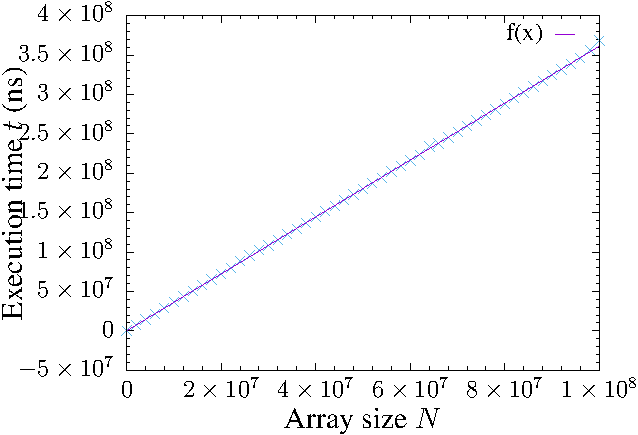
\includegraphics[scale=1.2]{../plots/lsearch_time.pdf}
  \caption{Comportamento assintótico da busca linear em relação ao tempo de execução médio (em milisegundos) a medida que o tamanho do arranjo sequencial $N$ aumenta.}
  \label{fig:lseach_time}
\end{figure} 


\section{Busca binária}

Os resultados da simulação do algoritmo de busca binária em suas versões iterativa e recursiva em arranjos sequenciais de tamanhos diferentes seguem abaixo. Fazendo um ajuste dos pontos da curva de ambas as implementações conseguimos determinar que o comportamento é logarítmico.
\begin{figure}[H]
  \centering
  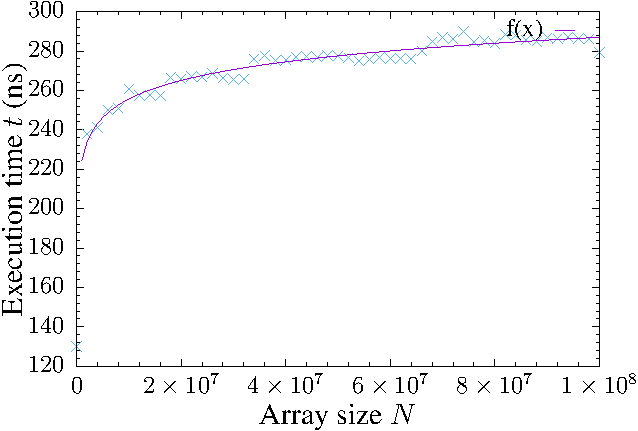
\includegraphics[scale=1.2]{../plots/bsearch_it_time.pdf}
  \caption{Comportamento assintótico da implementação iterativa da busca binária em relação ao tempo de execução médio (medido em nanosegundos).}
   \label{fig:bseach_it_time}
\end{figure}

\begin{figure}[H]
  \centering
  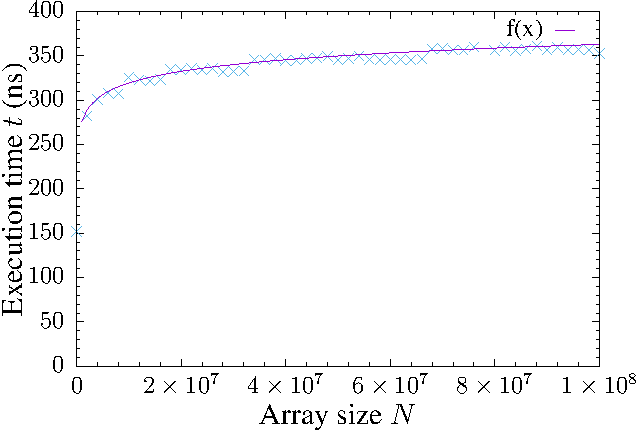
\includegraphics[scale=1.2]{../plots/bsearch_rec_time.pdf}
  \caption{Comportamento assintótico da implementação recursiva da busca binária em relação ao tempo de execução médio (medido em nanosegundos).}
  \label{fig:bseach_rec_time}
\end{figure} 


\section{Busca ternária}

Nesta subseção, apresentamos os gráficos de tempo de execução em função do tamanho do arranjo para a busca ternária em suas versões iterativa e recursiva. Fazendo um ajuste dos pontos da curva de ambas as implementações conseguimos determinar que o comportamento é logarítmico.
\begin{figure}[H]
  \centering
  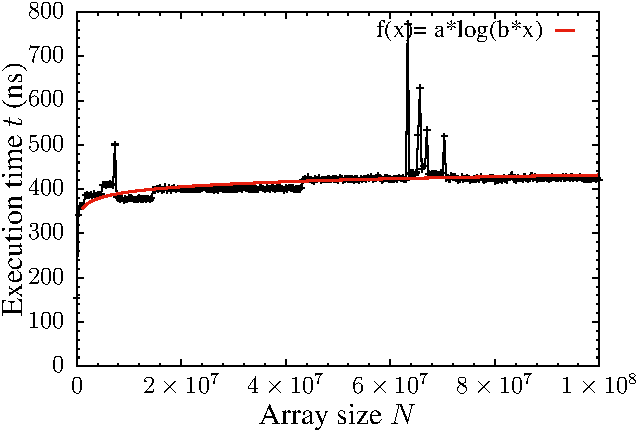
\includegraphics[scale=1.2]{../plots/tsearch_it_time.pdf}
  \caption{Comportamento assintótico da implementação iterativa da busca ternária em relação ao tempo de execução médio (medido em nanosegundos).}
  \label{fig:tseach_it_time}
\end{figure} 

\begin{figure}[H]
  \centering
  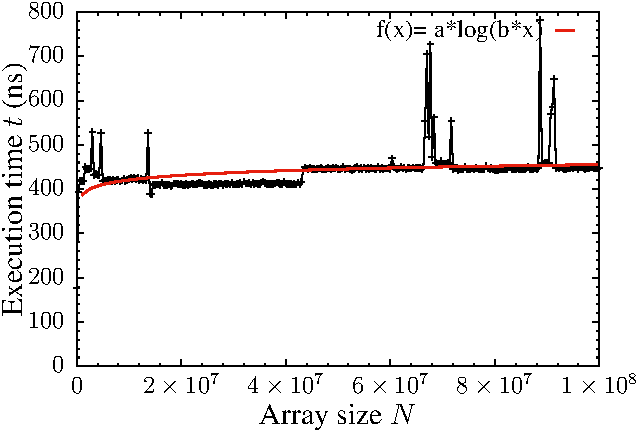
\includegraphics[scale=1.2]{../plots/tsearch_rec_time.pdf}
  \caption{Comportamento assintótico da implementação recursiva da busca ternária em relação ao tempo de execução médio (medido em nanosegundos).}
 \label{fig:tseach_rec_time}
\end{figure}

\section{{\it Jump search}}

Na figura abaixo temos o resultado da simulação do algoritmo {\it jump search} em arranjos sequenciais de tamanhos diferentes, onde o tempo de execução médio foi medido. Fazendo um ajuste dos pontos da curva conseguimos determinar que o comportamento assintótico é linear.
\begin{figure}[H]
  \centering
  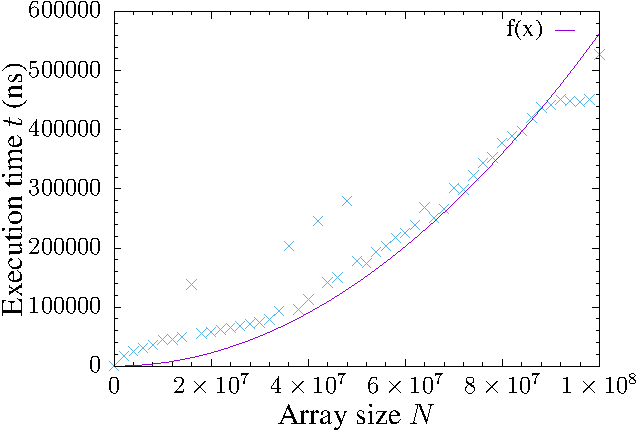
\includegraphics[scale=1.2]{../plots/jumpsearch_time.pdf}
  \caption{Comportamento assintótico da {\it jump search} em relação ao tempo de execução médio (medido em milisegundos) a medida que o tamanho do arranjo sequencial $N$ aumenta.}
  \label{fig:jumpsearch_time}
\end{figure} 

%\section{Busca de Fibonacci}

%\chapter{Resultados}

Nesta seção são analidos os resultados obtidos na seção anterior a fim de responder as perguntas que motivaram esse estudo.

\section{Algoritmos linear mais eficiente}

Determinar qual dos dois algoritmos lineares selecionados são mais eficientes (a busca linear ou a {\it jump search}).


\section{Implementação mais eficiente: recursiva ou iterativa?}

O segundo objetivo é determinar qual implementação é mais eficiente, a recursiva ou iterativa.



\section{Influência do tamanho da partição nos algoritmos de busca não lineares}

O terceiro, é determinar como o tamanho da partição influência nos algoritmos de busca não lineares.


\section{Diferenciação de algoritmos de classe de complexidade diferentes}

O quarto é determinar a partir de que momento algoritmos de classe de complexidade diferentes se diferenciam, comparando a busca linear com a binária.


\section{Cenários do algoritmo de Fibonacci}

Por fim, o quinto objetivo procura determinar se existe diferentes categorias de cenários de pior caso para o algoritmo de busca de Fibonacci.




%-------- APPENDIX -------------%
%\appendix
%\input{}


%-------- REFERENCES -----------%
%\input{referencias.tex} 
% or:

% Bibliografia
\renewcommand{\baselinestretch}{1}
\normalsize

%\bibliographystyle{amsalpha}
%\bibliographystyle{apsrev4-1}
%\bibliographystyle{nature}
%\bibliographystyle{thesnumb}
%\bibliographystyle{psuthesis}
%\bibliographystyle{phjcp}
%\bibliographystyle{ieee}
%\bibliographystyle{ieeetr}
%\bibliographystyle{phcpc}
%\bibliographystyle{phiaea}
%\bibliographystyle{h-physrev5}
%\bibliographystyle{phreport}
%\bibliographystyle{alpha} % like plain style but ref. markers are based on authors' initials and publication year (not 1,2,3...);
%\bibliographystyle{plain} % Entries are ordered alphabetically
%\bibliographystyle{unsrt} % Entries are ordered in the order they are first referenced
%\bibliographystyle{abbrv} % like plain style except that first names and names of journals and months are abbreviated;
\bibliographystyle{ieeetr} % merge unsrt and abbrv plus title in quotation marks
%\bibliographystyle{plainnat}

%\bibliography{refDis2014} %arquivo .bib
\renewcommand{\baselinestretch}{1.5}
\normalsize


\end{document}
